\documentclass{article}
\usepackage{hyperref}
\hypersetup{colorlinks=true,urlcolor=blue}
\usepackage{listings}
\usepackage{geometry}
\geometry{margin=1in}
\usepackage{graphicx}
\graphicspath{ {../} }
\lstset{language=Python,keywordstyle={\bfseries \color{purple}}}
\begin{document}
\title{BMI 203: Algorithms - Homework 3}
\author{Laurel Estes}
\maketitle
\section{Part I: Implementing Smith-Waterman and Evaluating Scoring Matrices}

\subsection{Smith-Waterman Implementation}
I implemented the Smith-Waterman algorithm primarily in the file \verb|align.py|, with a system of command-line argument parsing that allows it to be run with two single input files (the default), or raw terminal input (which comes in handy for testing on the fly), or batch input from a pair file (e.g. Pospairs.txt and Negpairs.txt). This last was the primary mode of usage for the remainder of the homework. Unlike some implementations available on the web, I chose to incorporate a record of traceback directionality into the process of filling the matrix--each cell in the alignment matrix is a 2-tuple, where the first index is the score of the cell and the second index is an integer representing the traceback direction from that cell--which increases its space utilization and may contribute to the slow running time of the algorithm in general.
\par Per recommendation in class, I attempted to use the \verb|numba| package with the \verb|@nb.jit()| decorator in front of highly-used functions, but this actually resulted in a dramatic slowdown of the overall running time, and the python kernel crashing/unable to quit with Ctrl+C. Some advice from Grayson was to try using \verb|@nb.jit(cache=True,nopython=True)|, but this did not resolve my issues and so the use of \verb|numba| was abandoned for this homework assignment.

\subsection{Optimal Gap Penalties for BLOSUM50}
Due to the long running time of the algorithm as implemented, I began searching for optimal gap penalty values first with a very coarse-grained method: I ran my false positive rate analysis on just the sequence pairs for which both sequences were under {\it N} characters in length, for increasing values of {\it N} (160 up to 250). Promising combinations of gap opening and gap extension scores were investigated more and more closely by increasing {\it N}, up until finally running the analysis for all 50 pairs of positive and negative sequences to make the final determination. 
\par Interestingly, even using the full 50 pairs of sequences, -3, -4 and -8 opening penalties and all 5 extension scores (1 through 5) were observed to have equally low false positive rates for a true positive rate of 0.7. From that subset, the combination of -4 as the gap opening penalty and 1 as the gap extension score was chosen mostly arbitrarily. Using all 50 negative and positive pairs, the lowest false positive passing rate I obtained was 0.5, which seems uncomfortably high; notably, running all sequences shorter than 250 characters (\~35 pairs out of the full 50) results in a rate of less than 0.2. More data from the tests used to arrive at these scores can be seen in the comments of the \verb|truefalse.py| file.
\par This method was not guaranteed to produce the most optimal gap penalty values, but, in talking with classmates who obtained similar values (predicated on the particulars of their false positive calculation method) suggests that it gets close, at least. More time spent reducing the running time of the algorithm would likely have enabled a more thorough search of the problem space.

\subsection{ROC Graphs for Provided Matrices}
Using the gap penalties of (-4,1) described in the previous subsection, the matrix with the lowest false positive passing rate when all the true positives pass is the BLOSUM50 matrix, by a very small margin. It also, by visual inspection, noticeably has the smallest area under the curve in the ROC graph.
\begin{figure}[h!]
\centering
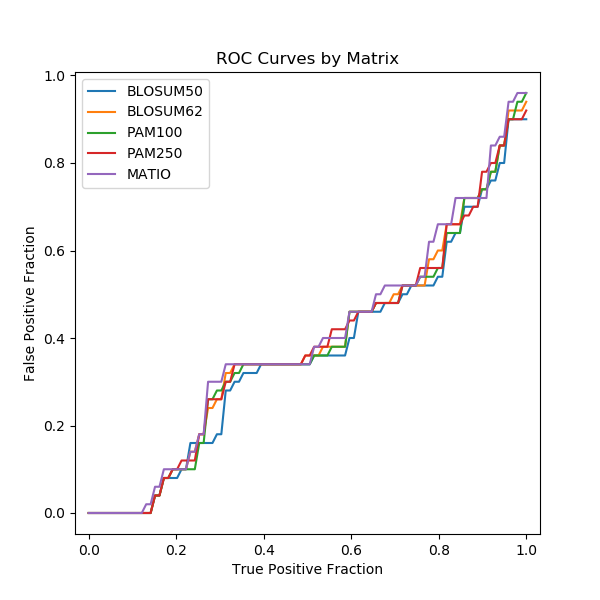
\includegraphics[width=0.8\textwidth]{ROC.png}
\end{figure}
\par At a true positive passing rate of 0.7, the false positive passing rates for the provided matrices (with the optimized gap penalties inserted!) are as follows:
\begin{center}
	\begin{tabular}{ l || l}
	Matrix & FP at TP=0.7 \\
	\hline
	BLOSUM50 & 0.48 \\
	BLOSUM62 & 0.50 \\
	PAM100 & 0.48 \\
	PAM250 & 0.48 \\
	MATIO & 0.52 \\
	\end{tabular}
\end{center}
Notably, in hindsight, perhaps using the optimized gap penalties for all of the provided matrices was {\it not} actually what the assignment intended, but the running time of the ROC analysis for the full 50 sequence pairs essentially prohibits retesting at this stage, if I want my homework submitted in a timely fashion.


\subsection{Normalizing Smith-Waterman Scores by Length}
If the raw Smith-Waterman alignment scores are normalized by dividing them by the length of the smaller of the two sequences being aligned, I obtained the ROC curves seen below.
\begin{figure}[h!]
\centering
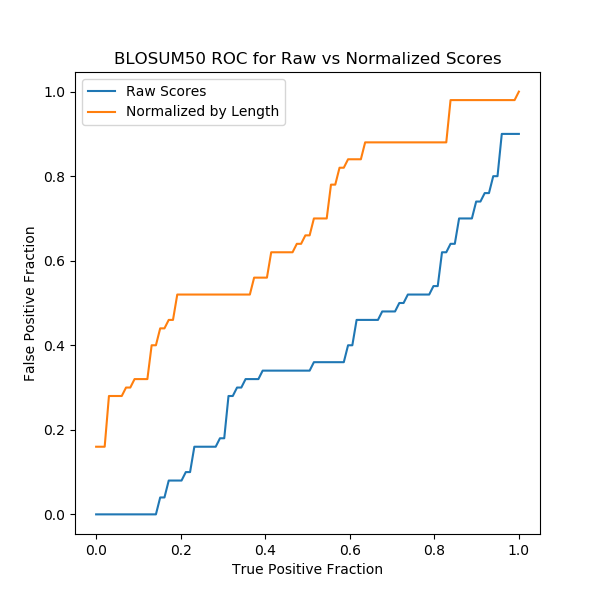
\includegraphics[width=0.8\textwidth]{ROC_Normalized.png}
\end{figure}
\par Interestingly, this normalization does {\it not} appear to improve the performance via the aforementioned metrics: the area under the curve is far larger, because the false positive passing rate for every true positive passing rate is much higher than for the non-normalized scores. If we divide the score by the sequence length, we are obtaining an alignment-quality-per-character score. It would seem that normalizing to this value would increase the scores of well-aligning shorter sequences and scale back the scores of moderately-well-aligning longer sequences. Intuitively, the longer the sequences that are being aligned, the harder it would be (by random chance) for them to align well; there is less information in a short sequence, so in one way of thinking about it, short sequences {\it should} have to align better, on a character-by-character basis, to reach the same score for alignment quality. Therefore, this may be the reason that the non-normalized Smith-Waterman scores are better at separating the true positives from the false positives in this example.

\section{Part II: Optimizing Scoring Matrices}

First, a note! I realized at this point that I had likely misinterpreted how gap penalty calculation was supposed to work up until this point, and that gap opening and gap extension penalties are {\it not} in fact part of the input matrix (as the ('N','*') and ('*','*') values, respectively), but are separate. This...essentially invalidates all of my earlier analysis, and in fact, I am still having issues with my Smith-Waterman code--apparently my tests were not thorough enough, and attempting to back-calculate the score from the output alignment sequences (e.g. `AAA*GC' + `AAATGC') results in a different value, despite my best troubleshooting efforts. In the interest of ever being able to finish this assignment, I am going to continue despite this discrepancy, just to go through the motions of applying my optimization algorithm to the BLOSUM50 and MATIO scoring matrices. 

\subsection{Optimization Algorithm}

For my optimization algorithm, I implemented a variation on a genetic algorithm, with two phases. Starting with a given base matrix and a scale factor (aka stepsize) along with the static positive and negative alignment pairs, in the first phase we create a library of matrices where each character pairing in the matrix is increased/decreased by the scale factor. Then the resulting library is screened against the positive and negative alignment pairs, and the subset (size chosen by user) with the highest objective function score is selected for hybridization in the second phase. For hybridization, a new matrix is created for every possible pair of matrices in the chosen subset and inherits the list of changes from the base matrix from both of its progenitor matrices. Then the hybrid matrices are screened and the best subset chosen, and the process repeated for the specified number of hybridization iterations per global iteration (aka number of phase two iterations for each phase one).
\par One drawback to this method is that the changes are always inherited as a single block: as one single ``chromosome'', in effect, with no crossing over. One could imagine a model where only some of the changes from each parent were transmitted, in a manner that still allowed for the total number of changes to increase or decrease. Also, in the current implementation, the step size is constant throughout the procedure; methods such as simulated annealing strongly suggest that the step size should decrease as the number of iterations increases, to allow the optimization to settle into the maximum instead of bouncing around it.

\subsection{Improvements to BLOSUM50}
The BLOSUM50 matrix starts out with an objective function score of []. Using my optimization algorithm ...
Repeating it with 10 global rounds, 3 merge iterations for each global round, a scale factor of 0.2, and a best subset size of 10 matricies also notably resulted in a best matrix with a score of only 2.0 out of 4. 


\subsection{Improvements to MATIO}
The MATIO matrix starts out with an objective function score of [], 



\section{Github Repository}
All of the code used in this assignment is on Github: \url{https://github.com/laueste/algorithms-ucsf-2019}
\end{document}
